\chapter{Risikoanalyse}

Die Risikoanalyse dient dazu, kritische Einflüsse innerhalb und außerhalb des Projektes zu identifizieren.
Für die STH App gilt vergleichbar zu allen anderen Projekten, dass der Projekterfolg nur mit begleitenden Risiken ermöglicht werden kann.
Für die Klassifizierung und Einschätzungen der Risiken dient eine Risikomatrix. Hierbei wird aufgezeigt, welche Risiken mit welcher Eintrittswahrscheinlichkeit und zugehöriger Auswirkung eintreten können.
Anhanddessen kann bewertet werden, welche Risiken besonders laufend beobachtet werden müssen und ob es Risiken gibt, die den Projekterfolg maßgeblich gefährden.

\section{Vorgehen Risikoanalyse}
Um eine Risikobewertungsmatrix erstellen und veranschaulichen zu können, benötigt es folgende Schritte.
Zunächst müssen die Risiken erkannt werden, die im Projekt auftreten können.
Dabei werden sowohl interne als auch externe Faktoren beleuchtet.
Zu den internen Risiken gehören z.B. Konflikte im Team und zu den externen Server Ausfallzeiten beim externen Dienstleister.
Hierbei ist zu beachten, dass mit jedem vorangegangenen Projektfortschritt auch neue Risiken hinzukommen können.
Daraufhin werden die Risiken nach ihrer Eintrittswahrscheinlichkeit klassifiziert.
Die Einordnung hilft dabei Risiken zu priorisieren.
Dabei werden Risiken mit hohen Eintrittswahrscheinlichkeiten genauer betrachtet und in Zukunft im Blick behalten.
Zuletzt werden die Risiken nach ihrer Auswirkung eingestuft.
Risiken mit hoher Eintrittswahrscheinlichkeit und hohen Auswirkungen können hierbei zum Scheitern des Projektes bzw\. zum Nichterfolg führen.
Deshalb ist es besonders wichtig diese Art von Risiken nicht nur zu beobachten, sondern kontinuierlich zu messen, welche Folgen der Eintritt haben kann.

\section{Grafische Darstellung Risikobewertungsmatrix}
Die Risikobewertungsmatrix für das Projekt STH App ist in der folgenden Abbildung (Nr einfügen) zu sehen.

\begin{figure}
	\caption[Risikomatrix]{Risikomatrix}
	\centering
	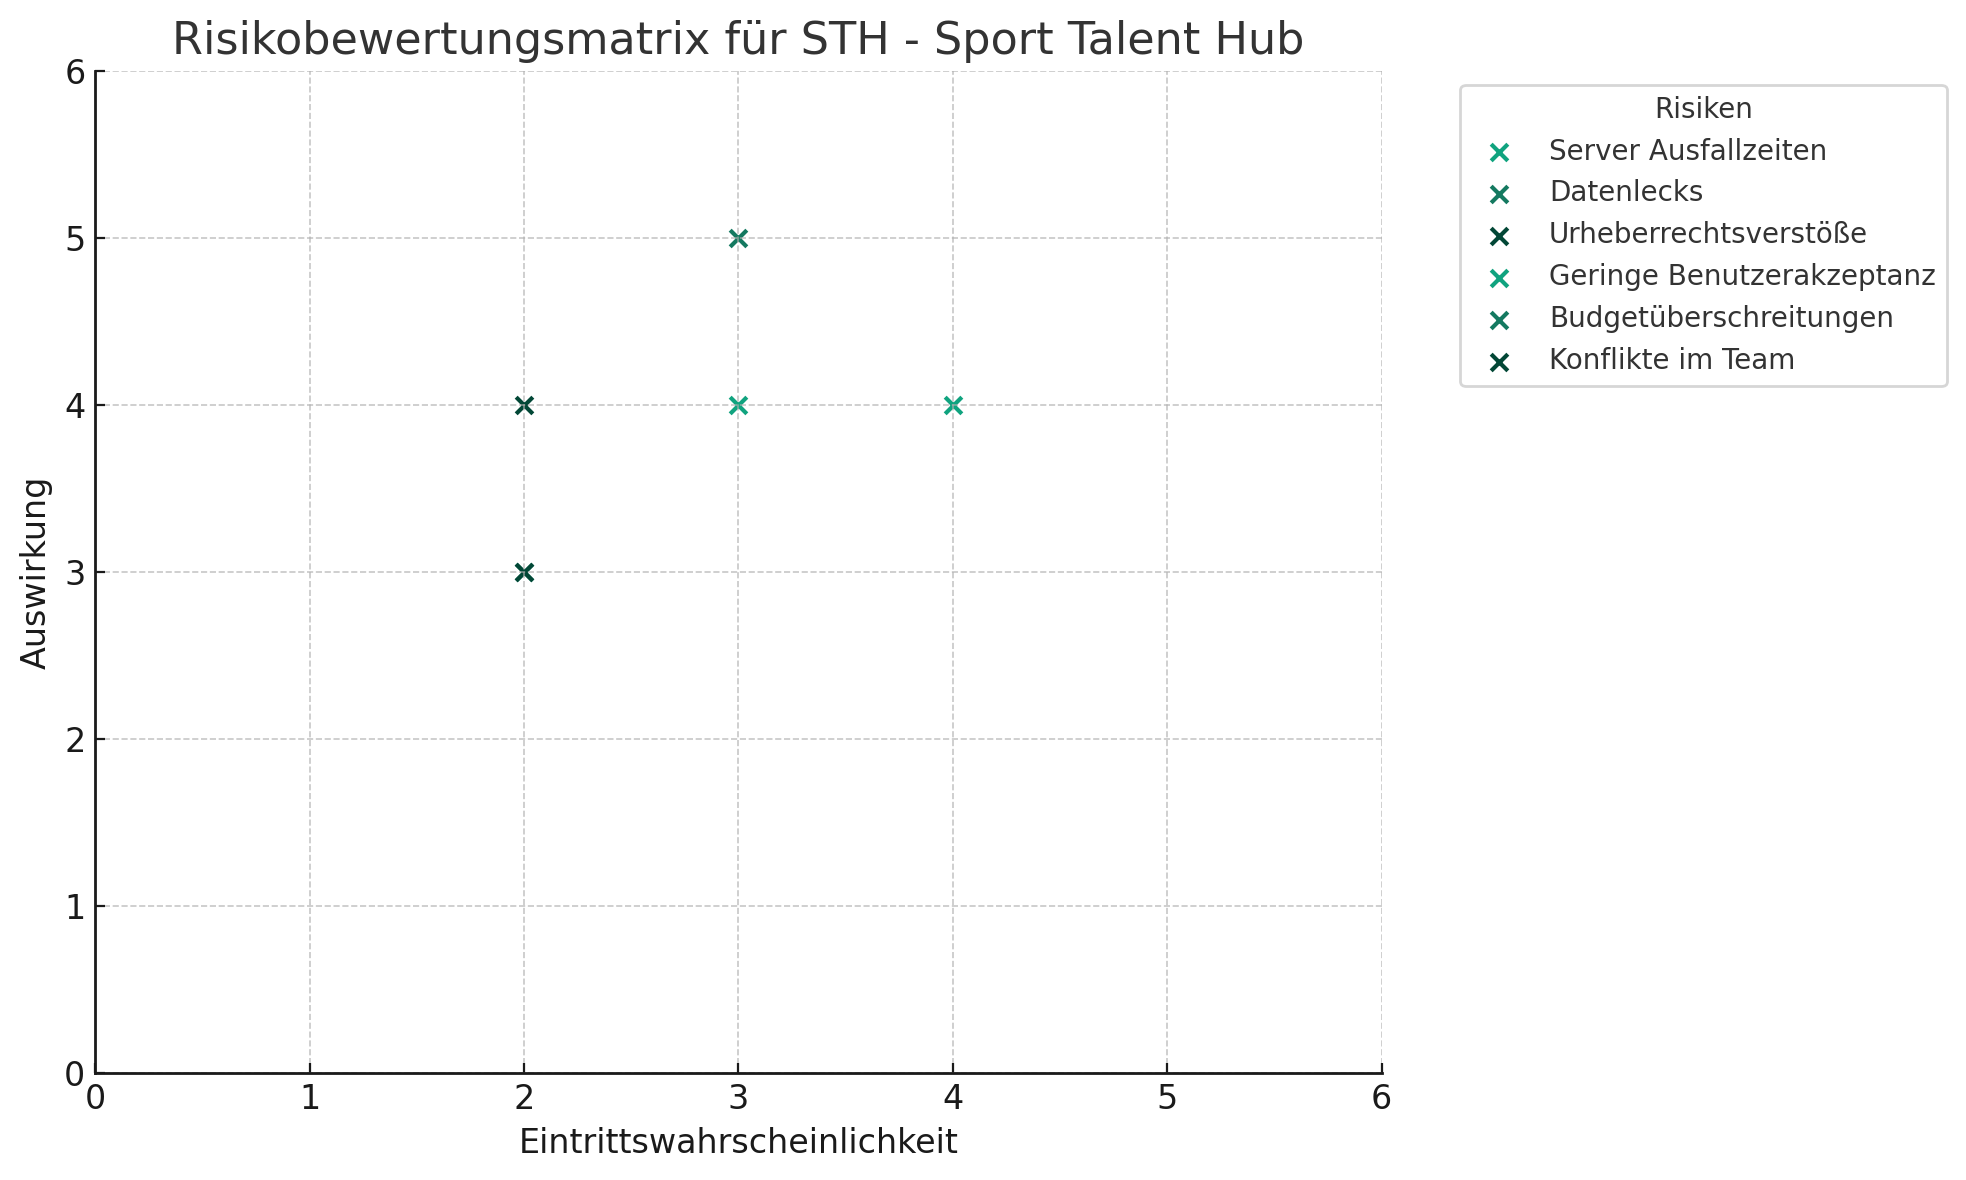
\includegraphics[width=\textwidth]{assets/figures/risikomatrix.png}
    \begin{flushleft}
		Quelle: Quelle Risikomatrix
	\end{flushleft}
\end{figure}

Für eine App mit diversen online Funktionen ist ein Server Ausfall fatal.
Deshalb wurde dieses Risiko als eines der mit am höchsten verbunden Auswirkungen klassifiziert.
Die Eintrittswahrscheinlichkeit bewegt sich hierbei im mittleren Bereich, da nach dem aktuellen Stand der Technik und der Rahmenverträge mit Dienstleistern bzw\. Rechenzentren bei einem Ausfall meist auf eine redundante Serverlandschaft ausgewichen werden kann.\newline
Ein Datenleck, welches durch einen Angriff auf die Backendsysteme entstehen kann, ist für den Erfolg und gleichzeitig für die Auswirkungen einer Smartphone-App schwerwiegend.
Innerhalb der STH App können sensible Daten eingegeben und abgespeichert werden, welche nicht an außenstehende gelangen dürfen.
Zudem sind die immensen Kosten bezüglich der Vertragsstrafen bei der Nichteinhaltung der DSGVO ein großes finanzielles Risiko.\newline
Ein weiteres Risiko für die Applikation sind Urheberrechtsverstöße.
Diese können auftreten, indem Nutzer Urheberrechtsgeschützte Inhalte veröffentlichen, welche nicht Ihnen gehören.
Eine Begünstigung der Urheberrechtsverstöße könnte auf die Applikation selbst zurückzuführen sein und damit finanziell intensive Vertragsstrafen auslösen.\newline
Eine geringe Benutzerakzeptanz kann durch ein vorher schlecht ausgearbeitetes UI/UX Konzept ausgelöst werden.
Die Eintrittswahrscheinlichkeit ist hierbei im mittleren Bereich, da es nicht einfach ist, den Nutzern ein qualitativ hochwertiges und gut durchdachtes User-Interface zu liefern.
Die Auswirkung liegt hierbei ebenso im mittleren Bereich, da das Design schnell angepasst werden kann.\newline
Die Budgetüberschreitung ist wie in fast jedem Projekt ein potenzielles Risiko, welches durchaus durch eine schlechte Planung auftreten kann.
Sobald die finanziellen Ressourcen ausgeschöpft sind, kann nicht mehr an der Applikation gearbeitet und weiterentwickelt werden.
Das könnte unter Umständen zu einem frühzeitigen Scheitern des Projektes führen.\newline
In jedem Projektteam ist immer ein gewisses Konfliktpotenzial vorhanden.
Dieses Risiko kann jederzeit und vor allem in Hochphasen wie z.B. kurz vor dem Start der Veröffentlichung der Applikation, auftreten.
Allerdings ist das Risiko durch eine gute Projektleitung gut einschätzbar und präventiv vermeidbar bzw\. zu lösen.